%%%%%%%%%%%%%%%%%%%%%%%%%%%%%%%%

% Author: Hugo Pereira
% Template available on github.com/hugopereira-eng
% Last modified: 09/06/2024

% In Preamble.tex you may find a list of custom commands defined to facilitate the ellaboration of the CV.

% This is an MIT licensed repository.

%%%%%%%%%%%%%%%%%%%%%%%%%%%%%%%%

\documentclass[a4paper,12pt]{article}

% Inputs
% -----------------------------Packages-------------------------------


\usepackage{titlesec}
\usepackage[usenames,dvipsnames]{color}
\usepackage{enumitem}
\usepackage[pdftex]{hyperref}
\usepackage{multirow}
\usepackage{graphicx}
\usepackage{multicol}
\usepackage{times}
\usepackage{tikz}
\usepackage{amsmath}
\usepackage{blindtext}


% ------------------------Custom Commands------------------------

% Education
% Inputs:
% #1 - University
% #2 - Start and end of studies
% #3 - Name of the degree
% #4 - Grade point average (optional)
\newcommand{\Education}[4]{
\vspace{-16pt}
\begin{table}[h!]
    \begin{tabular*}{\textwidth}{l@{\extracolsep{\fill}}r}
      \textbf{#1} & #2 \\ #3 & #4
    \end{tabular*} 
\end{table}
}

% Institution
% Inputs:
% #1 - Name of the institution
% #2 - Geographic location (optional)
\newcommand{\Institution}[2]{
    \begin{flushleft}
    \begin{tabular*}{\textwidth}{l@{\extracolsep{\fill}}r}
    \textbf{#1} & \textit{#2}
    \end{tabular*}
    \end{flushleft}  \vspace{-2em}
}

% Institution w/ Image
% Inputs:
% #1 - Logo
% #2 - URL (optional)
% #3 - Name of the institution
% #4 - Geographic location (optional)
\newcommand{\InstitutionWImage}[4]{
    \begin{flushleft}
    \begin{tabular*}{\textwidth}{l@{\extracolsep{\fill}}r}
 \href{#2}{\includegraphics[height=10pt]{#1}}~~\textbf{#3} & \textit{#4}
    \end{tabular*}
    \end{flushleft}  \vspace{-2em}
}

% Position
% Inputs:
% #1 - Name of the position
% #2 - Start and end dates 
\newcommand{\Position}[2]{
 \begin{flushleft}
    \begin{tabular*}{\textwidth}{l@{\extracolsep{\fill}}r}
      \quad \textit{#1} & \textit{#2}
    \end{tabular*}
    \end{flushleft} \vspace{-2em}
}


\newcommand{\ItemListStart}{\begin{itemize}\itemsep-2pt}

\newcommand{\ItemListEnd}{\end{itemize}\vspace{-10pt}}


\newcommand{\ItemWithTitle}[2]{
  \item \textit{#1}.~{#2}
}

\newcommand{\ItemWithoutTitle}[1]{
  \item{#1}
}


%--------------------------------Formatting---------------------------------

% Section title 
\titleformat{\section}{
  \vspace{-1em}\scshape\Large\bfseries
}{}{10pt}{}[\color{black}\titlerule]

% Margins 
\usepackage[
top    = 1.2cm,
bottom = 1.8cm,
left   = 1.2cm,
right  = 1.2cm]{geometry}

% URL font
\urlstyle{rm}  % Times New Roman

% Text
%\raggedbottom
%\raggedright % (uncomment to remove text justification)
\setlength{\tabcolsep}{0in}



%%%%%%%%%%%  CV STARTS HERE  %%%%%%%%%%


\begin{document}



%---------------------------------HEADER---------------------------------
\begin{minipage}{6.5cm}
\vspace{-1.5em}
\hspace{0.5cm}
\begin{tikzpicture}
    \clip (0,0) circle (2cm) node {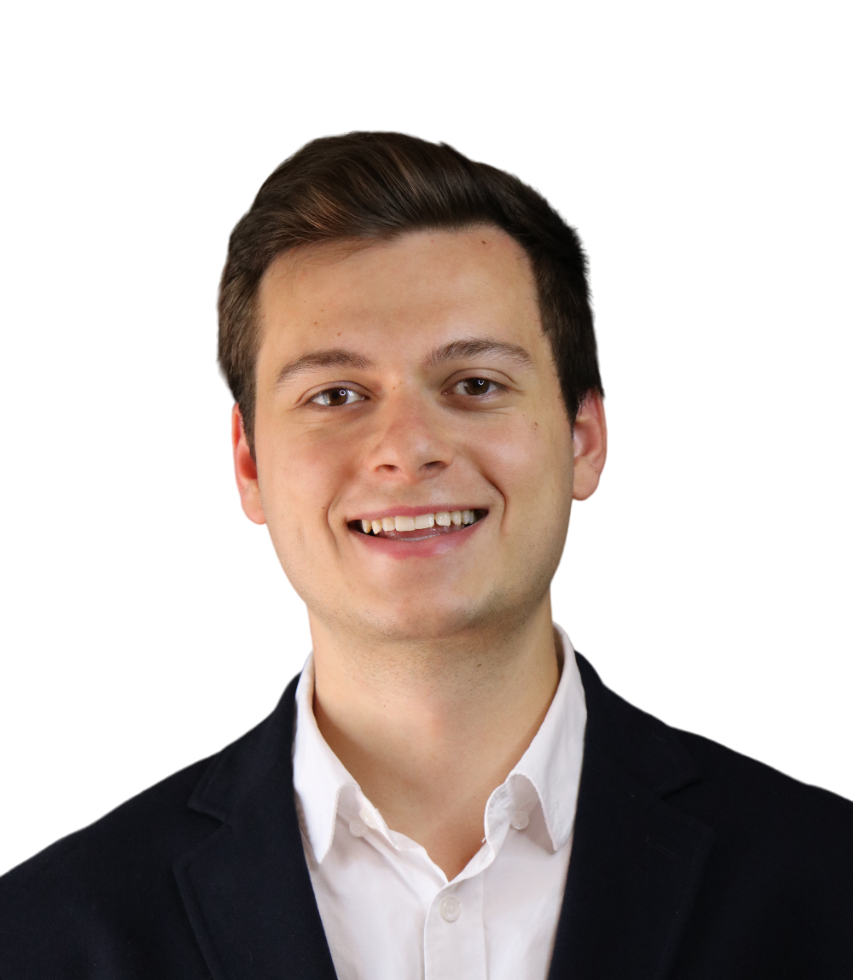
\includegraphics[scale=0.18]{Images/profile-2}};
\end{tikzpicture}
%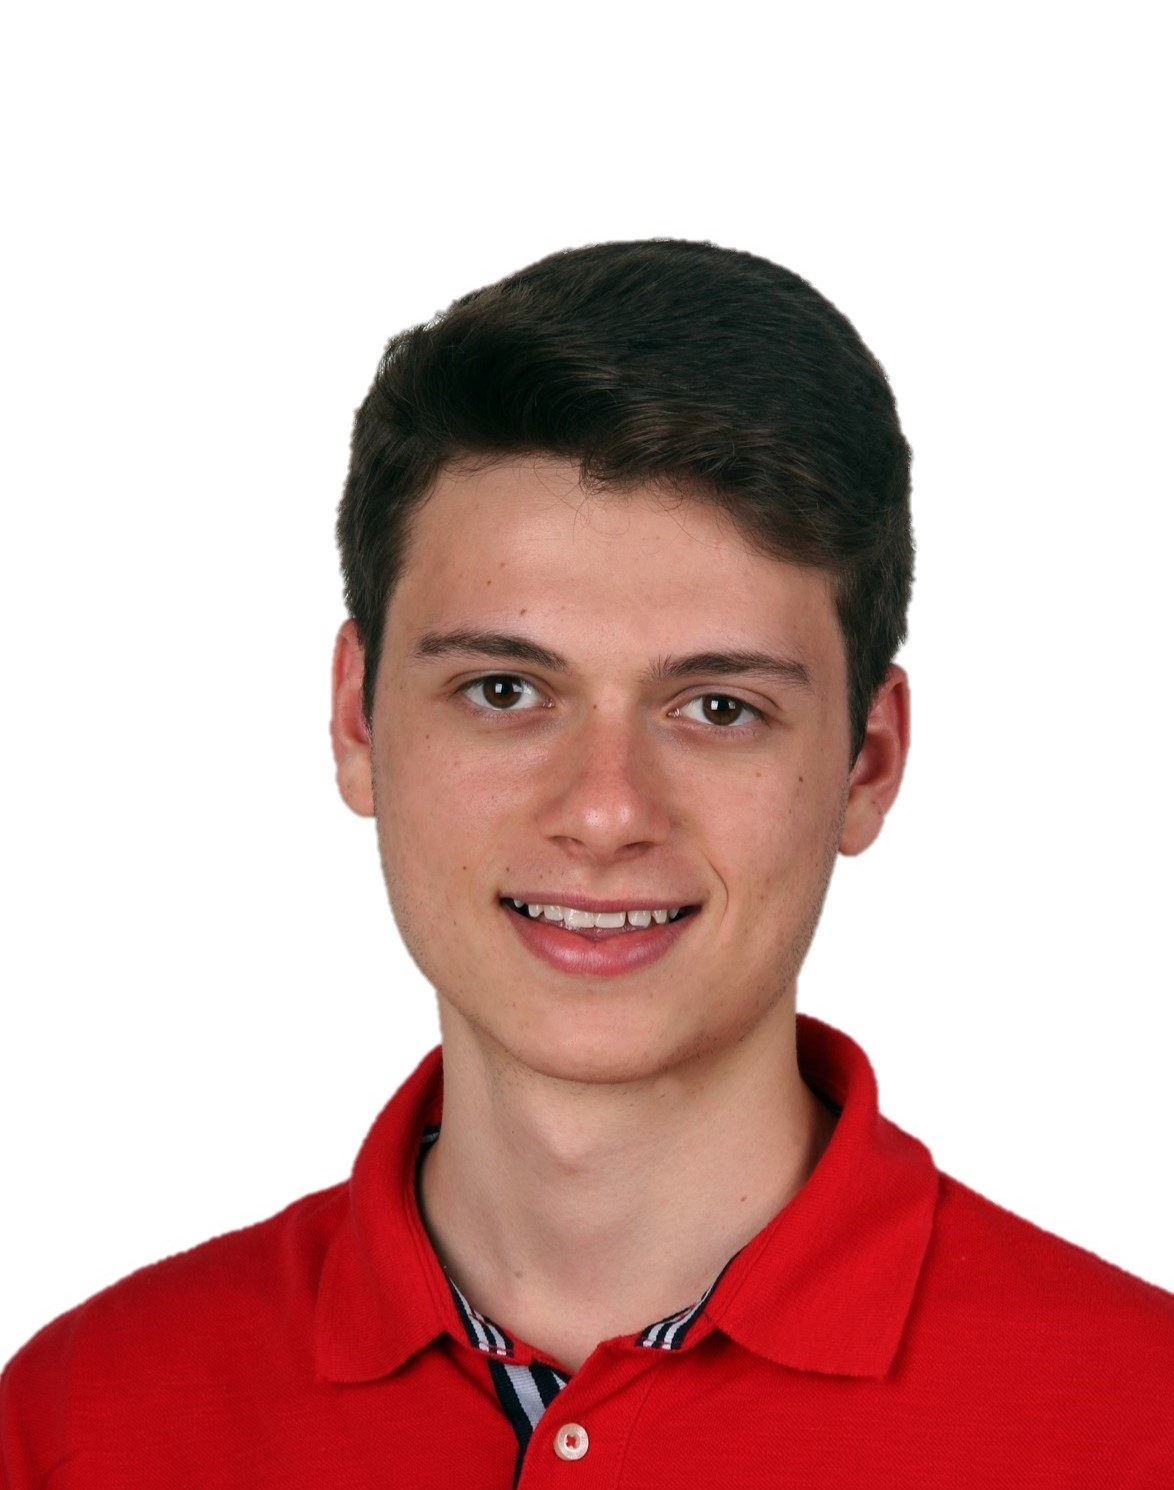
\includegraphics[scale=0.4]{Images/profile}  % uncomment for non-circular frame (and comment the 3 lines above)
\end{minipage}
\begin{minipage}{10.5cm}
\vspace{-1em}
\centerline{\Huge \textbf{Hugo Pereira}}
\vspace{8pt}
\centerline{\large \href{mailto:hugo.c.pereira@tecnico.ulisboa.pt}{hugo.c.pereira@tecnico.ulisboa.pt}}
\centerline{\large (+351) 96 33 62 767}
\centerline{\large Lisbon, Portugal} 
\vspace{8pt}
\href{https://www.linkedin.com/in/hugoacpereira/}{
\includegraphics[height=10pt]{Images/linkedin}~\footnotesize{linkedin.com/in/hugoacpereira/}}
\quad
\href{https://github.com/hugopereira-eng}{
\includegraphics[height=10pt]{Images/github}~\footnotesize{github.com/hugopereira-eng}} 
\end{minipage} 



%-------------------------------SUMMARY--------------------------------
%\section{Summary}
% - optional section
 


%------------------------------EDUCATION-------------------------------
\section{Education}

\Education{Instituto Superior Técnico, University of Lisbon}{2020 - 2022}{Master of Science in Aerospace Engineering~~(Control \& Systems branch)}{GPA:~19~/~20}

%\vspace{5pt}
 
\Education{Technical University of Denmark}{2020 - 2021}{Exchange Student }{GPA:~11~/~12}

%\vspace{5pt}

\Education{Instituto Superior Técnico, University of Lisbon}{2017 - 2020}{Bachelor of Science in Aerospace Engineering}{GPA:~17~/~20}

%\vspace{5pt}



%-----------------------------RESEARCH-EXPERIENCE-------------------------------
\section{Research Experience}

\InstitutionWImage{Images/ISR}{https://welcome.isr.tecnico.ulisboa.pt/}{Institute for Systems and Robotics}{Lisbon, Portugal}
\Position{Student Researcher~~(Full-time)}{Mar.~2022 - June~2023}
\ItemListStart
        \ItemWithoutTitle{Received a research fellowship to study the applications of embedded optimization in spacecraft attitude control for missions with agility requirements. Supervisors: Prof.~Pedro Batista and Dr.~Pedro Lourenço.}
        \ItemWithoutTitle{Crafted solutions for precise spacecraft steering in the presence of singularities, particularly those equipped with control moment gyros (CMGs). The solutions derived involve nonlinear control, convex optimization and advanced algebra, providing novel insights into the problem of CMG singularity avoidance.}
        \ItemWithoutTitle{Developed a 6 DoF simulator for model-in-the-loop testing of a spacecraft in LEO subject to environmental disturbances.}
        \ItemWithoutTitle{Worked towards my master's thesis titled \textit{"A Convex Allocation Framework for Singularity Avoidance in Control Moment Gyro Clusters"}, which was awarded the grade of 20 out of 20.}
\ItemListEnd 



%-----------------------------WORK-EXPERIENCE-------------------------------
\section{Work Experience}
\InstitutionWImage{Images/GMV}{https://www.gmv.com/en-es/}{GMV}{Lisbon, Portugal}
\Position{GNC Engineer~~(Full-time)}{July~2023 - Present}
\ItemListStart
        \ItemWithoutTitle{GNC engineer based in the Lisbon office. Responsible for developing guidance, navigation and control algorithms for space missions ranging from very low Earth orbit to deep space.}
        \ItemWithoutTitle{Designed attitude control algorithms for the ARIEL telescope, an exoplanet observation mission operated by ESA, scheduled for launch in 2030.}
        \ItemWithoutTitle{Derived synthesis models for reusable launch vehicles within the FTC-CRE (Fault Tolerant Control of Clustered Rocket Engines) project.}
\ItemListEnd


\InstitutionWImage{Images/UAVision}{https://www.uavision.com/}{UAVision}{Torres Vedras, Portugal}
\Position{Summer Intern~~(Full-time)}{June~2021 - July~2021}
\ItemListStart
        \ItemWithoutTitle{Short-term internship where I contributed to the design of a signal demodulation program for an Emergency Position Indicating Radio Beacon. The system, developed in collaboration with other interns, was sketched in GNU Radio and written in Python.}
\ItemListEnd



%---------------------EXTRACURRICULAR-ACTIVITIES------------------------
\section{Extracurricular Activities}

\InstitutionWImage{Images/FST}{https://www.fstlisboa.com/}{Formula Student Lisboa}{Lisbon, Portugal}
\Position{Autonomous Systems Engineer~~(Part-time)}{Sep.~2021 - Sep.~2022}
\ItemListStart
        \ItemWithoutTitle{Developed autonomous driving algorithms, using ROS/C++, for a driverless Formula car. The autonomous pipeline encompasses machine learning for point cloud processing, state estimation via Kalman filtering, simultaneous localization and mapping (SLAM), and model predictive control (MPC).}
        \ItemWithoutTitle{Specifically, my responsibilities included implementing data association methods for pose estimation, optimizing the mapping of the track, formulating nonlinear control strategies for path following, and validating point cloud processing algorithms.}
        \ItemWithoutTitle{Worked under the agile scrum methodology and followed an optimized workflow through CI/CD.}
        \ItemWithoutTitle{Competitions: Formula Student Germany 2022, $3^{rd}$ place in the Driverless Cup; Formula Student Spain 2022, $1^{st}$ place in the Driverless Cup.}
\ItemListEnd


\InstitutionWImage{Images/DanSTAR}{https://www.danstar.dk/}{Danish Student Association for Rocketry}{Copenhagen, Denmark}
\Position{Avionics Systems Engineer~~(Part-time)}{Nov.~2020 - Oct.~2021}
\ItemListStart
        \ItemWithoutTitle{Member of the electronics department that was in charge of the electrical systems of the rocket. I designed, tested and soldered multiple PCBs for an STM32-based flight computer.}
        \ItemWithoutTitle{Led the development of the rocket's telemetry system from conceptual design to on-board implementation. Established a communication link based on LoRa technology that operated within a 9~km range.}       
         \ItemWithoutTitle{Carried out robust flight simulations using the OpenRocket software, which resulted in a predicted apogee error of less than 3\%.}
         \ItemWithoutTitle{Competition: European Rocketry Challenge 2021, Portugal; Received the 9~km flight category award; The team set the altitude world record for collegiate bi-liquid rocketry with an apogee of 6545~m AGL.}
\ItemListEnd


\InstitutionWImage{Images/AeroTec}{https://aerotec.pt/}{Aerospace Engineering Students Group $\vert$ AeroTéc}{Lisbon, Portugal}
\Position{UAV Engineer~~(Part-time)}{Oct.~2018 -  June~2020}
\ItemListStart
        \ItemWithoutTitle{Part of the UAV-ART project, whose goal was to design an autonomous fixed-wing aircraft to navigate through predefined waypoints. In my first year with the team, I participated in the design and construction of the UAV. In the second year, I took part in the development of the flight controller, which involved PID control, data filtering, path planning, sensor fusion, and system identification algorithms. The simulations were carried out in \textsc{Matlab}/\textsc{Simulink} and the on-board controller was implemented in an RPi.}
        \ItemWithoutTitle{Gave workshops about rocketry to high school and college students. These consisted of a hands-on experience in planning, building and launching a small rocket made of cheap conventional materials.}
\ItemListEnd



%----------------------------------SKILLS------------------------------------
\section{Skills Summary}

\vspace{-10pt}

\begin{align*}
&\text{\textbf{Languages}} &&\text{English (C1 certificate), Portuguese (Native)}\\
&\text{\textbf{Programming}} &&\text{C++, C, \textsc{Matlab}, Python} \\
&\text{\textbf{Frameworks}} &&\text{PyTorch, TensorFlow, Scikit-learn, Pandas, NumPy} \\
&\text{\textbf{Software}} &&\text{\textsc{Simulink}, KiCad, OpenRocket, SolidWorks}\\
&\text{\textbf{Tools}} &&\text{Git, \textsc{LaTex}, Microsoft Office}\\
&\text{\textbf{Platforms}} &&\text{Linux, Windows, ROS, STM32, PIC24, Arduino}\\
&\text{\textbf{Miscellaneous}} &&\text{Soldering, Driving License}
\end{align*}


\break
%----------------COMPLEMENTARY-TRAINING---------------------
\section{Complementary training}

\ItemListStart
\ItemWithTitle{Ladybird Guide to Spacecraft Communications Training Course, 2022, ESA Academy}{Selected to attend a remote spacecraft communications course featuring live sessions given by ESA experts.}
\ItemWithTitle{Summer course in Robotics, University of Twente, Aug.~2019}{On-site summer camp in Robotics at the University of Twente in the Netherlands. This consisted of a hands-on experience with real-time robotics systems and included a group project centered on Arduino manipulation.}
\ItemListEnd



%--------------------------VOLUNTEERING-----------------------------
\section{Volunteering}

\Institution{Erasmus Student Network, DTU section}{Feb. 2021 - June 2021}
\ItemListStart
\ItemWithoutTitle{Member of a multinational team of volunteers whose goal is to facilitate the integration of international students in the local community.}
\ItemWithoutTitle{Organized social events and provided general support and guidance for exchange students.}
\ItemListEnd



%-------------------------------AWARDS----------------------------------
\section{Honors and Awards}

\begin{description}[font=$\circ$]
\itemsep-2pt 
\item {Academic Excellence, Instituto Superior Técnico, 2021/2022}
\item {Outstanding Performance at EuRoc 2021, DTU Blue Dot, Oct. 2021}
\item {Academic Merit, Instituto Superior Técnico, 2017/2018, 2019/2020}
\item {Best Student Award, Escola Secundária Marquesa de Alorna, 2015/2016, 2016/2017}
\end{description}



%----------------------------ACTIVITIES---------------------------------
\section{Hobbies and Activities}

\begin{description}[font=$\circ$]
\itemsep-2pt
\item {Training four times a week, alternating between running, climbing and gym workouts.}
\item {Learning to play the guitar. Currently attending weekly guitar lessons.}
\item {Practiced athletics as a federated athlete for 8 years (2009-2017) while competing at the national level.}
\end{description}



%----------------------------CERTIFICATES-----------------------------
%\section{Certificates}
%
%\begin{description}[font=$\circ$]
%\itemsep-2pt 
%\item {Online Ladybird Guide to Spacecraft Communications Training Course, 2022, ESA Academy}
%\item {Drone Simulation and Control, 2020, MOOC TÉCNICO}
%\item {European BEST Engineering Competition, 2018, BEST}
%\end{description}



\end{document}